\documentclass{anstrans}
%%%%%%%%%%%%%%%%%%%%%%%%%%%%%%%%%%%
\title{A Simple Reactor-Model Game to Assist Conceptual Learning}
\author{Robert W.~Carlsen,$^{*}$ Matthew J.~Gidden$^{\*}$}

\institute{
$^{*}$University of Wisconsin, Nuclear Engineering Dept., 1500 Engineering Dr., Madison, WI
}

\email{rcarlsen@wisc.edu \and gidden@wisc.edu}

%%%% packages and definitions (optional)
\usepackage{graphicx} % allows inclusion of graphics
\usepackage{booktabs} % nice rules (thick lines) for tables
\usepackage{microtype} % improves typography for PDF

\newcommand{\SN}{S$_N$}
\renewcommand{\vec}[1]{\bm{#1}} %vector is bold italic
\newcommand{\vd}{\bm{\cdot}} % slightly bold vector dot
\newcommand{\grad}{\vec{\nabla}} % gradient
\newcommand{\ud}{\mathop{}\!\mathrm{d}} % upright derivative symbol

\begin{document}
%%%%%%%%%%%%%%%%%%%%%%%%%%%%%%%%%%%%%%%%%%%%%%%%%%%%%%%%%%%%%%%%%%%%%%%%%%%%%%%%
\section{Introduction}

Microsoft Word can be a finicky beastie. \LaTeX\ abstracts content from
formatting, allowing the user to let a style file such as this take care of
uppercasing the section headings, spacing the paragraphs, and shuffle around
the figures.

The \SN\ equations were developed by Carlson \cite{Car1953}. Another
paper is cited here \cite{Lar2008}.

%%%%%%%%%%%%%%%%%%%%%%%%%%%%%%%%%%%%%%%%%%%%%%%%%%%%%%%%%%%%%%%%%%%%%%%%%%%%%%%%
\section{Methodology}

Equations look exceedingly pretty. Here is a 3-D, monoenergetic, steady-state
transport equation with isotropic scattering and an isotropic extraneous source:
\begin{subequations} \label{eqs:fullTransport}
\begin{multline} \label{eq:fullTransportVol}
  \vec{\Omega}\vd \grad \psi(\vec{x}, \vec{\Omega})
  + \sigma(\vec{x}) \psi (\vec{x}, \vec{\Omega})
\\ =
  \frac{\sigma_s(\vec{x})}{4\pi} \int_{4\pi} \psi(\vec{x},\vec{\Omega}')
  \ud\Omega' + \frac{q(\vec{x})}{4\pi}
  \equiv \frac{1}{4\pi} Q(\vec{x}) \,,
\end{multline}
inside $\vec{x} \in V$, $\vec{\Omega} \in 4\pi$, with an incident boundary
condition
\begin{equation} \label{eq:fullTransportBndy}
  \psi(\vec{x}, \vec{\Omega}) = \psi^b(\vec{x}, \vec{\Omega}) \,,
 \quad \vec{x} \in \partial V, \ \vec{\Omega} \vd \vec{n} < 0\,.
\end{equation}
\end{subequations}

%%%%%%%%%%%%%%%%%%%%%%%%%%%%%%%%%%%%%%%%%%%%%%%%%%%%%%%%%%%%%%%%%%%%%%%%%%%%%%%%
\section{Experiments and Results}

The results were interesting, so interesting in fact that we have decided to
present them here.

\subsection{Attenuation}

\subsection{Criticality and Burnup}

\begin{figure}
    \centering
    
\includegraphics{reactor-thermal-setup.png}
    \caption{Supercritical thermal reactor setup.}
    \label{fig:thermal-setup}
\end{figure}

\begin{figure}
    \centering
    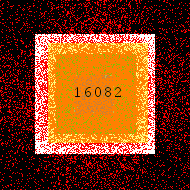
\includegraphics{reactor-thermal-1min.png}
    \caption{Supercritical thermal reactor continues to grow its neutron population. }
    \label{fig:thermal-on}
\end{figure}

\begin{figure}
    \centering
    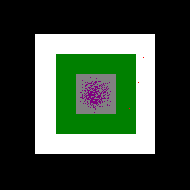
\includegraphics{reactor-thermal-after.png}
    \caption{After shutdown, the thermal reactor exhibits non-uniform burnup in the fuel. }
    \label{fig:thermal-after}
\end{figure}

\subsection{Subcritical Multiplication}

\begin{figure}
    \centering
    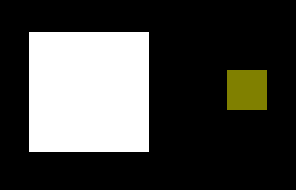
\includegraphics{scatter-setup.png}
    \caption{Reference setup for measuring neutron equilibrium in a scattering medium.}
    \label{fig:scatter-setup}
\end{figure}

\begin{figure}
    \centering
    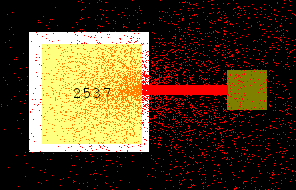
\includegraphics{scatter-equil.png}
    \caption{Reference scattering setup reaches an equilibrium neutron population of about 2500 neutrons when fed by a constant streaming source.}
    \label{fig:scatter-equil}
\end{figure}

\begin{figure}
    \centering
    
\includegraphics{subcrit-mult-setup.png}
    \caption{Fuel was introduced into the scattering medium creating a subcritical multiplication configuration.}
    \label{fig:subcrit-setup}
\end{figure}

\begin{figure}
    \centering
    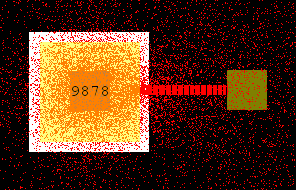
\includegraphics{subcrit-mult-equil.png}
    \caption{Subcritical multiplication reaches an equilibrium neutron population of about 10,000 neutrons when fed by a constant neutron source.}
    \label{fig:subcrit-equil}
\end{figure}

For those who like equations in their papers, \LaTeX\ is a good choice. Here is
an equation for the Marshak diffusion boundary condition:
\begin{equation} \label{eq:marshak}
  4 J^- = \phi + 2 D \vec{n} \vd \grad \phi \,.
\end{equation}
If we so choose, we can effortlessly reference the equation later.

Another paragraph starts with Eq.~\eqref{eq:marshak} and sets $J^-$ to zero, a
vacuum boundary condition:
\begin{equation*}
  0 = \phi + \frac{2}{3} \frac{1}{\sigma} \vec{n} \vd \grad \phi \,.
\end{equation*}

The extrapolation distance is $2/3$. A more detailed asymptotic analysis yields
an extrapolation distance of about $0.71045$.

Later on, we can include a table, even one that spans two columns such as
Table~\ref{tab:widetable}.
%%%%%%%%%%%%%%%%%%%%%%%%%%%%%%%%%%%%%%%%
\begin{table*}[htb]
  \centering
\begin{tabular}{llllllllll}\toprule
      & $\phi_T(0)$      & $\phi_T(10)$      & $\phi_T(20)$      &
      $\phi_D(0)$      & $\phi_D(10)$      & $\phi_D(20)$      & $\rho$      &
      $\varepsilon$      & $N_\text{it}$
\\ \midrule
$c=0.999$  & 0.9038 & 20.63 & 31.24 & 0.9087 & 20.63 & 31.23 & 0.2192 & $10^{-7}$ & 15
\\
$c=0.990$  & 0.3675 & 13.04 & 24.7 & 0.3696 & 13.04 & 24.69 & 0.2184 & $10^{-7}$ & 15
\\
$c=0.900$  & 0.009909 & 4.776 & 17.64 & 0.009984 & 4.786 & 17.63 & 0.2118 & $10^{-7}$ & 14
\\
$c=0.500$  & $6.069\times 10^{-5}$ & 2.212 & 15.53 & 6.213$\times 10^{-5}$ & 2.239 & 15.53 & 0.2068 & $10^{-7}$ & 13
\\
\bottomrule
\end{tabular}
  \caption{This is an example of a really wide table which might not normally
  fit in the document.}
  \label{tab:widetable}
\end{table*}

%%%%%%%%%%%%%%%%%%%%%%%%%%%%%%%%%%%%%%%%%%%%%%%%%%%%%%%%%%%%%%%%%%%%%%%%%%%%%%%%
\section{Conclusions}

The included ANS style file and this clear example file are a panacea for
the hours of headache that invariably results from formatting a document in
Microsoft Word.

%%%%%%%%%%%%%%%%%%%%%%%%%%%%%%%%%%%%%%%%%%%%%%%%%%%%%%%%%%%%%%%%%%%%%%%%%%%%%%%%
\section{Acknowledgments}
This material is based upon work supported a Department of Energy Nuclear
Energy University Programs Graduate Fellowship.

%%%%%%%%%%%%%%%%%%%%%%%%%%%%%%%%%%%%%%%%%%%%%%%%%%%%%%%%%%%%%%%%%%%%%%%%%%%%%%%%
\bibliographystyle{ans}
\bibliography{bibliography}
\end{document}

